\section{Methods}

% ------------------------------------
\subsection{Score Function}
\label{score function}

% ------------------------------------
\subsection{Random}

% ------------------------------------
\subsection{Greedy}

% ------------------------------------
\subsection{Minimax Search}

% ------------------------------------
\subsection{Reinforcement Learning}
\subsubsection{Monte-Carlo Tree Search}
MCTS (Monte-Carlo Tree Search), a well-known algorithm used in Alpha-GO, could handle large state space problems and complex decision trees. Here we apply MCTS to classical draught games. As shown in figure \ref{fig:mcts}, the MCTS algorithm builds the search tree during the iterations of four steps: Selection, Expansion, Simulation, and Backpropagation. To build the tree, we define our tree structure with tree nodes. For each node, we store the visit time, win time, and parent and children. For the current node, we could use the rule of draught to find all possible movements as the children of the node. Then we explain the details of the four steps. 
\begin{figure}[t]
    \centering
    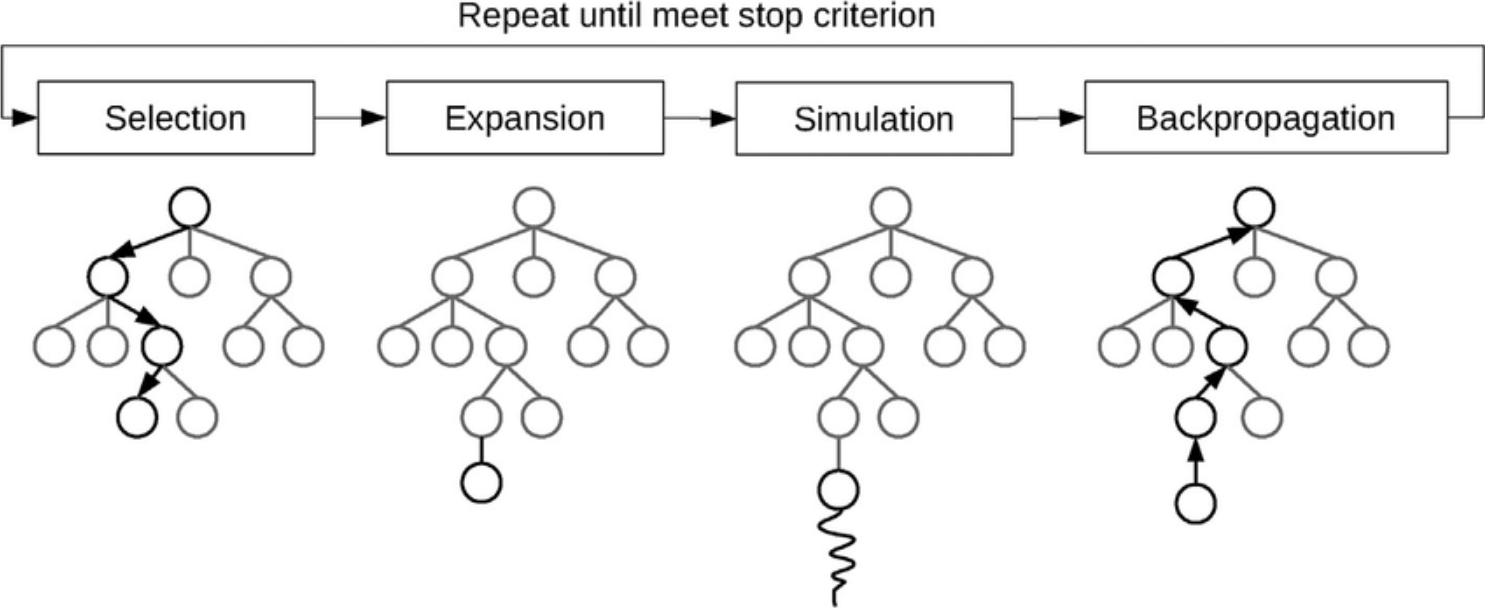
\includegraphics[width=\linewidth]{figures/mcts.png}
    \caption{Illustration of the MCTS algorithm steps}
    \label{fig:mcts}
\end{figure}
\begin{enumerate}
    \item \textbf{Selection} We start from the root node of the search tree, representing the current state of the game, where we use board class to store the current game state. Then we use the UCT (Upper Confidence Bound for Tree) selection policy to select child nodes. The UCT is an application of UCB, and the value can be obtained by $$\mathop{\arg\max}\limits_{v' \in {\rm children \, of} v} \dfrac{Q(v')}{N(v')} + c \sqrt{\dfrac{2 lnN(v)}{N(v')}}$$ where $v$ represents for the parent node, $v'$ is one of the child node of $v$, $N$ is the nodes' visit time, and $Q$ is the quality value of the current node. Note that c is chosen as $\frac{1}{\sqrt{2}}$ as an empirical constant. Each time we select the node with maximum UCT value, by selecting iteratively, we find the leaf node of the search tree that hasn't been fully expanded as a result of the selection step. 
    \item \textbf{Expansion} After selecting a leaf node, we generate child nodes for the current node of possible future states, and then we add these nodes as the child nodes of the leaf node. 
    \item \textbf{Simulation} After Expansion, we perform a simulation of one of the added child nodes. Here we randomly choose actions in the simulation step to estimate the possible final state of the current node. Note that for the speed of the agent, we will limit the max actions step, so if the node needs large steps to get the final state, we will end this step ahead and regard the player that has more pieces as the winner. 
    \item \textbf{Backpropagation} Lastly, we perform backpropagation through the tree to update all parent nodes of the search path. We update the visit times and the reward of win or lose to each node.
\end{enumerate}
As for an MCTS agent, we first initialize a state class to store the current state of the game, then we perform the four steps for fixed iterations. After building the tree for search, we choose the best child of the current node by finding the maximum layouts and return the corresponding best action. With a larger number of iterations, the tree is built more richly, thus the agent will be more intelligent. However increasing the number of iterations will also result in longer inference time, so a balance between iterations and intelligence is important. 

% ------------------------------------
\subsubsection{Q-Learning}
\subsubsection{Approximate Q-Learning}